\chapter{AWS Amplify}

Das folgende Kapitel beschreibt die Architektur und die Implementierung der geplanten Anwendung mit AWS Amplify.

\section{Architektur}

Für die Architektur wird zunächst die Lösungsstrategie vorgestellt. Darauf folgen die Bausteinsicht, die Laufzeitsicht sowie die Verteilungssicht.

\subsection{Lösungsstrategie}

Die Architektur lässt sich in Präsentation, Logik und Datenhaltung aufteilen, welche durch unterschiedliche Cloud-Dienste und Frameworks abgebildet sind.
\begin{itemize}
  \item Präsentation
    \begin{itemize}
      \item React.js
      \item amplify-js
    \end{itemize}
  \item Logik
    \begin{itemize}
      \item AppSync
      \item Lambda
      \item Cognito
      \item Elemental MediaConvert
      \item EventBridge
      \item IAM
    \end{itemize}
  \item Datenhaltung
    \begin{itemize}
      \item DynamoDB
      \item S3
      \item Cognito
      \item IAM
      \item Amplify Hosting
    \end{itemize}
\end{itemize}

Die Dienste Cognito und IAM befindet sich zugleich in der Logik als auch in der Datenhaltung, da dort neben der Authentifizierung und Autorisierung auch die Benutzer persistiert werden.

Durch die ausschließliche Verwendung interner Dienste von \ac{AWS}, keiner Eigenentwicklungen für die Benutzerverwaltung und den vorgegebenen Technologien sind die Rahmenbedingungen für dieses Projekt nicht missachtet, so dass die beiden Technologien weiterhin vergleichbar sind.

Als nächstes werden Lösungsansätze, um die nichtfunktionalen Anforderungen, auch Qualitätsziele genannt, zu erreichen:

\begin{description}
   \item[Verfügbarkeit] Amplify bietet für Frontend und Backend ein Zero-Downtime Deployment.
   \item[Skalierbarkeit] Durch die Serverless-Architektur skalieren Dienste automatisch innerhalb der \ac{AWS}-Cloud. Die DynamoDB-Datenbank ist serverless und muss deshalb auch nicht skaliert werden.
   \item[Analysierbarkeit] Durch den Einsatz von CloudWatch können Anfragen für Lambda-Funktionen nachvollzogen werden.
   \item[Interoperabilität] Durch den Einsatz von AppSync ist mit GraphQL eine einheitliche Schnittstelle sichergestellt. Außerdem werden die GraphQL-Queries und Mutations automatisch über eine Codegenerierung für das Frontend erstellt.
   \item[Backups] Durch den Einsatz von DynamoDB Backup and Restore werden automatisierte Backups für die letzten 35 Tage aufgesetzt.
   \item[Wiederherstellbarkeit] Das von DynamoDB Backup and Restore erstellte Backup für die Datenbank DynamoDB kann direkt eingespielt werden.
\end{description}

\subsection{Bausteinsicht}

Die Architektur ist unterteilt in Frontend (Präsentationsschicht) und Backend (Logik- und Datenhaltungsschicht). Das Frontend wird nicht näher beschrieben, da Amplify dieses vollständig verwaltet. Das Backend besteht aus Stacks, welche zugleich den Code als auch die Infrastruktur repräsentieren. Diese werden im folgenden Abschnitt dargestellt:
\begin{itemize}
  \item{Der \textit{RootStack} enthält alle darunterliegenden Stacks sowie Ressourcen zum Deployment von Amplify.}

  \item{Der \textit{ApiStack} besteht aus den Diensten AppSync und DynamoDB. AppSync besteht aus einer GraphQLApi, die ein GraphQLSchema enthält. Außerdem nutzt AppSync Resolver, um ein Mapping über VTL zur DynamoDB-Tabelle zu ermöglichen. Um eine Verbindung zu einer Lambda-Funktion zu ermöglichen, existiert auch mindestens eine DataSource.}

  \item{Der \textit{AuthStack} regelt die Authentifizierung und Autorisierung von Benutzern über den Dienst Cognito. Dieser besteht aus einem UserPool und einem IdentityPool und den entsprechenden IAM-Rollen und Policies. Des weiteren besteht der Stack aus einem UserPoolClient, über welchen Anfragen auf Cognito erfolgen können. Amplify definiert auch weitere Lambda-Funktionen, um zusätzliche Logik für die Authentifizierung zu ermöglichen.}

  \item{Der \textit{AuthUserPoolGroupStack} dient zur Verwaltung der zusätzlichen UserPoolGroup für Administratoren.}

  \item{Der \textit{StorageStack} dient zur Speicherung der Videos. Dieser enthält einen S3-Bucket sowie eine dazugehören Policy, welchen es Benutzern ermöglicht, Dateien in eigene Ordner hochzuladen sowie andere Ordner lesen zu dürfen. Die Policy unterscheidet zwischen öffentlichen, geschützten und privaten Geltungsbereichen.}

  \item{Der \textit{FunctionLayerStack} bündelt die Node.js-Module als Lambda-Layer, den die weiteren Lambda-Funktionen nutzen.}

  \item{Der \textit{FunctionCreateVideoStack} übernimmt die Erstellung eines Videos in Form einer Lambda-Funktion. Außerdem erstellt der Stack in MediaConvert ein JobTemplate und eine Queue. Des Weiteren definiert der Stack die nötige Policy und Rolle, um der Lambda-Funktion die Zugriffe auf andere Dienste zu ermöglichen.}

  \item{Der \textit{FunctionVideoConvertedStack} besteht aus einer EventBridge-Regel, die bei einer Konvertierung eines Videos aufgerufen wird. Außerdem wird eine Lambda-Funktion mit der nötigen Policy und Rolle erstellt.}

  \item{Der \textit{FunctionCreateLinkStack} besteht aus einer Lambda-Funktion und der nötigen Rolle und Policy, um einen signierten zeitlich begrenzt gültigen Video-Link zu erstellen.}
\end{itemize}

Die Stacks \textit{RootStack}, \textit{ApiStack}, \textit{AuthStack}, \textit{AuthUserPoolGroupStack} und \textit{StorageStack} erstellt Amplify selbst. Die restlichen Stacks sind selbst erstellte bzw. angepasste Plugins, da die Dienste nicht vollständig in Amplify vorhanden sind.

\subsection{Laufzeitsicht}

Die Laufzeitsicht beschreibt die wichtigsten Prozesse und wie die Bausteine miteinander interagieren.

\subsubsection{Auflisten, Aktualisieren und Löschen eines Videos}

\begin{figure}
  \centering
  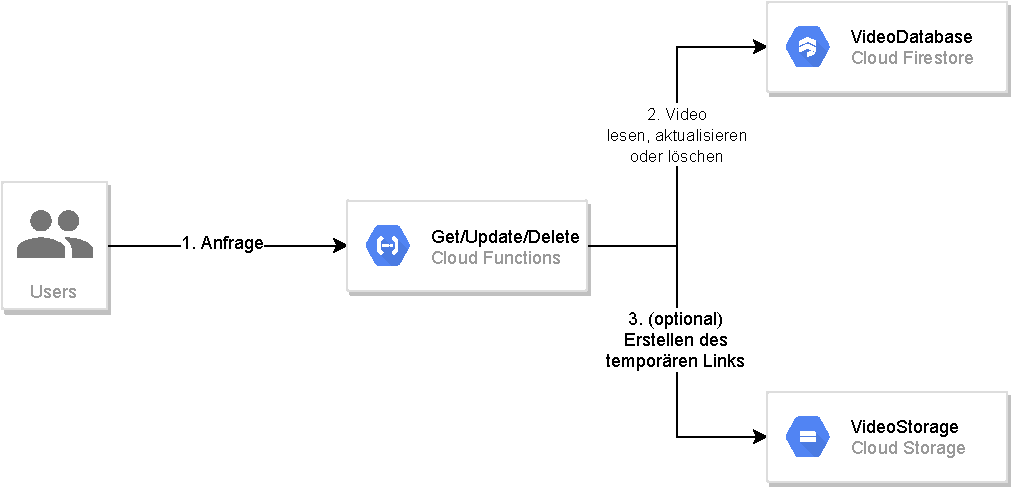
\includegraphics[width=0.75\columnwidth]{5_aws-amplify/laufzeitsicht_1.pdf}
  \caption{AWS Amplify - Laufzeitsicht - Auflisten, Aktualisieren und Löschen eines Videos}
  \label{Amplify:laufzeitsicht1}
\end{figure}

\autoref{Amplify:laufzeitsicht1} stellt den Prozess dar, wie Videos von Nutzern aufgelistet, aktualisiert oder gelöscht werden. Dieser wird im folgenden Abschnitt näher erläutert:
\begin{enumerate}
  \item{Der Nutzer stellt eine Anfrage mittels GraphQL und dem JSON Webtoken.}
  \item{AppSync autorisiert den Nutzer und holt die Gruppenzugehörigkeit des Nutzers.}
  \item{Der Resolver leitet die Anfrage unter Berücksichtigung der Gruppenzugehörigkeit des Nutzers an DynamoDB weiter. Die nötigen Datenbankoperationen werden über DynamoDB ausgeführt.}
\end{enumerate}

Zusätzlich dazu müssen signierte temporäre Links erstellt werden, um die Sicherheit zu gewährleisten. Dieser Ablauf, der in \autoref{Amplify:laufzeitsicht2} dargestellt wird, enthält noch eine zusätzlich Abfrage auf S3, um den Link zu erstellen.

\begin{figure}
  \centering
  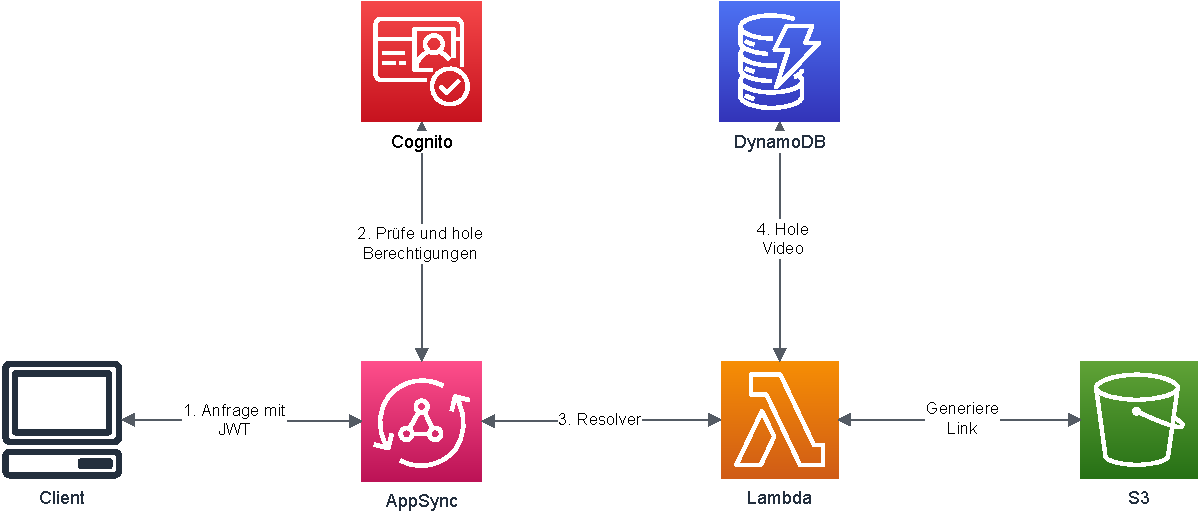
\includegraphics[width=1\columnwidth]{5_aws-amplify/laufzeitsicht_3.pdf}
  \caption{AWS Amplify - Laufzeitsicht - Erstellen von Links}
  \label{Amplify:laufzeitsicht2}
\end{figure}

\subsubsection{Erstellen eines Videos}

\autoref{Amplify:laufzeitsicht3} stellt den Prozess dar, wie ein Video erstellt wird.
\begin{enumerate}
  \item{Zunächst lädt der Nutzer das Video in den S3-Bucket hoch. Die Policy des S3-Buckets verwaltet den korrekten Zugriff auf die Ressource. Die hochgeladene Datei landet in einem privaten Ordner, der außerhalb des Backends ausschließlich für den Besitzer des Objekts aufrufbar ist. Das ist der Nutzer, der das Video hochgeladen hat.}
  \item{Erst dann erstellt der Nutzer eine Anfrage mittels GraphQL und dem JSON Webtoken.}
  \item{AppSync autorisiert den Nutzer und holt die Gruppenzugehörigkeit des Nutzers.}
  \item{Der Resolver führt die verknüpfte Lambda-Funktion aus.}
  \item{Die Funktion kopiert die hochgeladene Datei in einen weiteren Ordner, so dass der Besitzer diese nicht mehr verändern kann. Die hochgeladene Datei im Ursprungsordner wird daraufhin gelöscht.}
  \item{Die Funktion erstellt das Video in der DynamoDB-Tabelle.}
  \item{Die Funktion führt den MediaConvert-Job aus, um das Video mit dem Wasserzeichen zu versehen.}
  \item{Ist die Konvertierung abgeschlossen, benachrichtigt die EventBridge eine weitere Lambda-Funktion, welche das Video dann freischaltet.}
\end{enumerate}

\begin{figure}
  \centering
  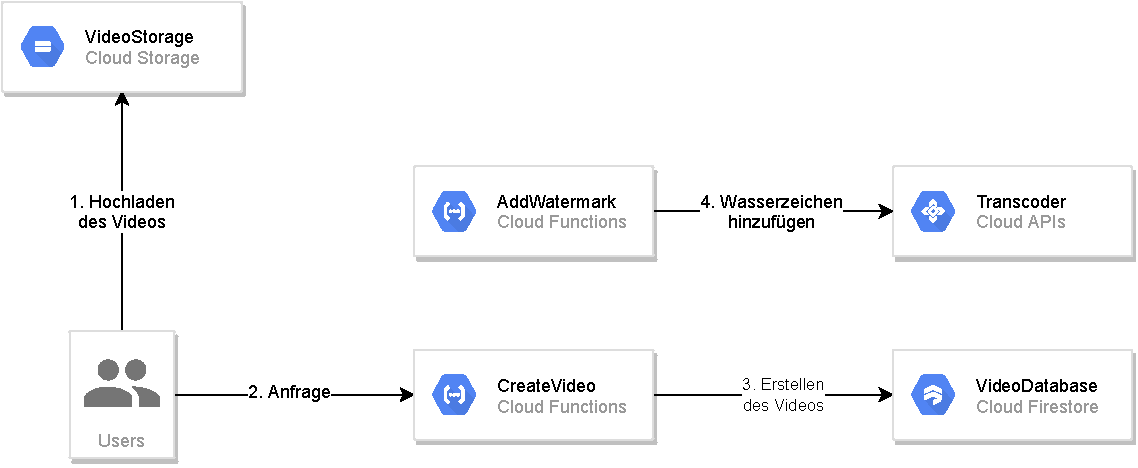
\includegraphics[width=1\columnwidth]{5_aws-amplify/laufzeitsicht_2.pdf}
  \caption{AWS Amplify - Laufzeitsicht - Erstellen eines Videos}
  \label{Amplify:laufzeitsicht3}
\end{figure}

\subsection{Verteilungssicht}

Die Verteilungssicht beschreibt, wie die Bausteine in \ac{AWS} über Stacks verteilt werden. Amplify bündelt die Verteilung des Backends und des Frontends über eine Pipeline. Diesen Sachverhalt stellt \autoref{Amplify:verteilungssicht} dar.

\begin{figure}
  \centering
  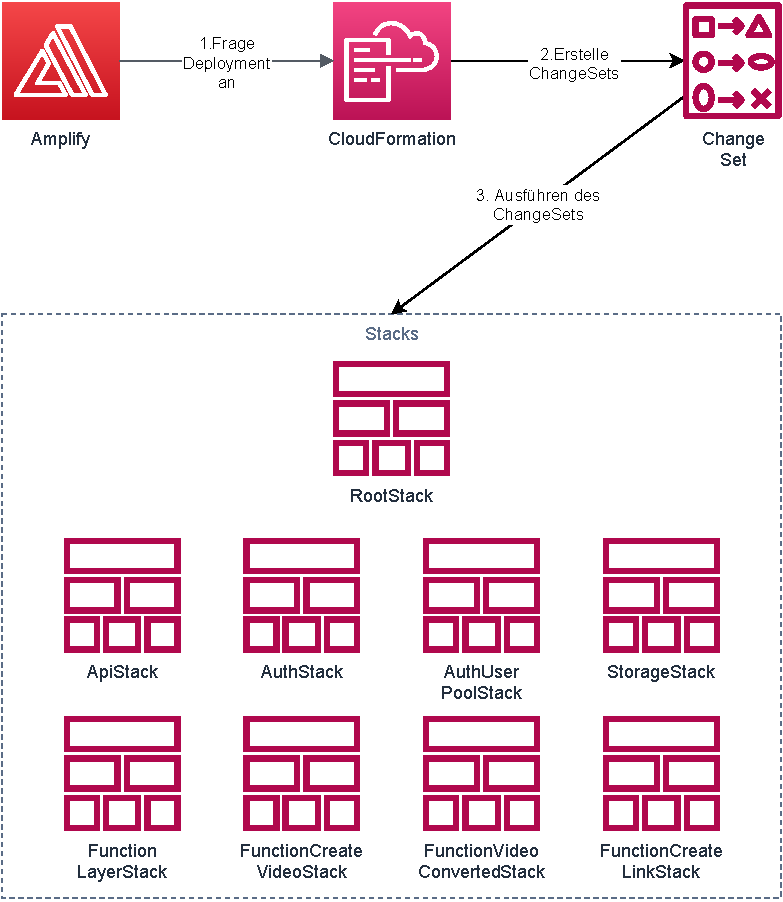
\includegraphics[width=0.75\columnwidth]{5_aws-amplify/verteilungssicht.pdf}
  \caption{AWS Amplify - Verteilungssicht}
  \label{Amplify:verteilungssicht}
\end{figure}

Amplify verteilt das Backend über die CloudFormation mittels Stacks. Außerdem werden nur Stacks und keine NestedStacks genutzt, was die Fehleranalyse vereinfacht. Um eine neue Änderung in das System einzuspielen, erzeugt die CloudFormation ein ChangeSet, welches die Differenz aus dem aktuellen Stand in der Cloud und dem gewünschten Zielzustand ist. Wenn beim Aktualisieren der Stacks ein Fehler auftritt, erfolgt ein Rollback.

Das Frontend wird separat, also nicht über Stacks, verteilt. Dazu nutzt Amplify einen gebündelten Dienst, der über die CloudFront läuft. Letzterer kann allerdings als Black-Box betrachtet werden, da der Entwickler diesen nur durch die Konfiguration beeinflussen kann.

\section{Implementierung}

Die Implementierung in Amplify unterscheidet die Themen Infrastruktur, Backend und Frontend. Zwar liegt die Infrastruktur-Definition und der Backend-Code vereint in Plugins, die sich im selben Repository befinden, dennoch können sie separat betrachtet werden.

\subsection{Infrastruktur}

Für die Infrastruktur müssen einige Plugins verändert werden, da Amplify nicht alle Dienste direkt als fertige Plugins anbietet. Dies erfolgt daher durch eine initiale Erstellung mittels der Amplify CLI sowie einer nachträgliche Anpassung des Plugins. Die hier vorgestellten Plugins beziehen sich alle auf die Kategorie \textit{function}. Weitere Anpassungen in den Kategorien \textit{auth}, \textit{api} oder \textit{storage} waren nicht nötig.

Das CloudFormation-Template für das Plugin \textit{createVideo} wird um die nötigen Ressourcen für die Video-Konvertierung erweitert. Das Plugin \textit{videoConverted} wird um eine Regel erweitert, die zum Abschluss der Video-Konvertierung die Lambda-Funktion ausführt. Alle Plugins, bei denen Lambda-Funktionen auf andere Dienste zugreifen, erhalten zusätzliche Berechtigungen für den aufzurufenden Dienst im Template.

Einen Ausschnitt der Anpassungen am Plugin \textit{createVideo} zeigt \autoref{lst:AmplifyCreateVideo}. Hier ist die Ergänzung der Attribute \textit{MediaConvertJobTemplate} und \textit{MediaConvertQueue} und deren Definitionen zu sehen. Wichtig dabei ist, dass der Name des Diensts jeweils das aktuelle Environment beinhaltet. Sonst wäre es nicht möglich über verschiedene Git-Branches zu arbeiten, da die Namen eindeutig sein müssen. Das Attribut \textit{SettingsJson}, welches hier nicht vollständig dargestellt ist, speichert die Definition für die Video-Konvertierung.

\lstinputlisting[
  language=JavaScript,
  extendedchars=true,
  basicstyle=\footnotesize\ttfamily,
  showstringspaces=false,
  showspaces=false,
  numbers=left,
  numberstyle=\footnotesize,
  numbersep=9pt,
  tabsize=2,
  breaklines=true,
  showtabs=false,
  caption={Amplify Custom Plugin},
  label=lst:AmplifyCreateVideo
]{\srcloc/amplify/cf-create-video.json}

\subsection{Backend}

Für die Backend-Logik wird ein GraphQL-Schema in AppSync benötigt. Dieses stellt die nötigen Verbindungen zu den Lambda-Funktionen und der DynamoDB her. \autoref{lst:AmplifyGraphQLSchema} zeigt dieses Schema.

Die beiden Mutationen \textit{createVideo} und \textit{createPresignedVideoLink} rufen mit den Funktionsparametern die definierte Funktion auf. Der Funktionsname enthält das aktuelle Environment, damit mehrere Git-Branches möglich sind.

Des Weiteren wird ein Video-Type definiert. Über den \textit{@model}-Parameter werden alle Aktionen bis auf \textit{Create} und \textit{onCreateVideo} ausgeschlossen, da diese selbst programmiert und nicht über VTL-Resolver zu DynamoDB abgebildet werden. Über den \textit{@auth}-Parameter werden die benötigten Zugriffskontrollen etabliert. Die Definition sorgt dafür, dass nur der Besitzer des Videos sowie ein Administrator ein Video löschen oder aktualisieren darf. Die Aktionen Lesen und Erstellen sind immer erlaubt. Aus diesem Schema erstellt AppSync automatisch eine GraphQL-API, die das Frontend für Abfragen auf die Videos nutzen kann. Die API bietet auch Filtermöglichkeiten an, um die Suche nach dem Video-Titel abzubilden.

\lstinputlisting[
  language=JavaScript,
  extendedchars=true,
  basicstyle=\footnotesize\ttfamily,
  showstringspaces=false,
  showspaces=false,
  numbers=left,
  numberstyle=\footnotesize,
  numbersep=9pt,
  tabsize=2,
  breaklines=true,
  showtabs=false,
  caption={Amplify GraphQL-Schema},
  label=lst:AmplifyGraphQLSchema
]{\srcloc/amplify/schema.graphql}

Die Lambda-Funktionen sind in Node.js programmiert und nutzen die \textit{aws-sdk}, um weitere Dienste wie DynamoDB, S3 oder MediaConvert anzusprechen. Um den Cold-Start der Lambda-Funktionen möglichst kurz zu halten, sind alle Node.js-Packages in einem externen Lambda-Layer ausgelagert.

\subsection{Frontend}

Das Frontend ist in React.js entwickelt. Relevant für diese Arbeit ist, dass das Frontend die Amplify-Bibliotheken nutzt. Diese Bibliothek wird über die \textit{aws-config.js} konfiguriert, welche die Domains zu Cognito, AppSync und zu dem S3-Bucket beinhaltet. Folgende Komponenten werden aus Amplify genutzt:

\begin{description}
  \item[Api] Diese Komponente nutzt GraphQL, um Anfragen an AppSync zu senden und zu empfangen. Die AWS CLI kann die nötigen GraphQL-Befehle dafür bei einer Aktualisierung der API automatisiert erstellen. Außerdem kann die Komponente über einen Socket bei Änderungen in GraphQL wie \textit{onUpdate} oder \textit{onDelete} die nötigen Sockets aufzusetzen.
  \item[Auth] Diese Komponente regelt die Funktionalität für die Authentifizierung von Benutzen. Insbesondere kann die Komponente vor die Anwendung einen Login-Schutz inklusive einer Funktion zur Zurücksetzung des Passworts und der Erstellung eines neuen Accounts setzen.
  \item[Storage] Diese Komponente bietet dem Nutzer die Möglichkeiten, Videos über S3 zu lesen und zu schreiben.
\end{itemize}